\section{Project analysis and System requirements}
\phantomsection

\subsection{Problem Definition}
A photographer tasked with year long time-lapse usually spends its friday checking on the time-lapses. He would usually use an application like TeamViewer or another Remote Desktop application to connect to the computer that has the cameras connected to. He would have to manually check if the desktop application is still running and if it had any failures. If he is lucky enough, he might have written a script that opens the application on startup and program the mouse to start the time-lapse again from the last index, only if no additional pop-ups appear in the meantime. On the other hand, if the time-lapse is very expensive, say it's a very expensive experiment that requires a few weeks time-lapse, then the photographer would have for each camera an open remote desktop to see if it is still working.

It becomes exponentially difficult to automate this entire process for different models of cameras. In big enterprises usually the photographer is given a set o company owned cameras, which often come from different brands: Canon, Nikon, Sony, Pentax, Olympus, etc. Each brand usually comes with its own specific software, so it becomes next to impossible to write an all purpose reliable script to automate a time-lapse composed of multiple different cameras.

Taking continuous high quality time-lapses is one of the most challenging work that can be done by a photographer.

\subsection{Project Analysis}
DSLR Camera Controller is a tool which aims to provide easy access and management of cameras, supporting a wide range of models, through a web browser. The main features are:
\begin{enumerate}
    \item Live preview;
    \item Take a picture;
    \item Camera configuration;
    \item Failure strategy:
    \begin{itemize}
        \item Send email;
        \item Hard reset;
        \item Reboot system after N failures;
    \end{itemize}
    \item Time-lapse scheduling;
    \item File transfer;
    \item Photo name patterns:
    \begin{itemize}
        \item Time (timestamp, hour, minute, day, year, etc);
        \item Capture index;
        \item Camera serial number;
        \item Camera name;
        \item Time-lapse name;
    \end{itemize}
\end{enumerate}

\subsubsection{Failure strategy}
A camera can fail because of a variety of reasons. Some models, automatically go to into sleep mode when the connected computer does not send any commands for an hour. This happens very often, as some time-lapses usually happen during the working days. Another common case is when the local workers simply unplug the device, or trip on the cable. Other times the power is simply cut off for a brief period of time, causing some confusion on some models. So choosing a failure strategy is very important to reduce the time the user has to spend on the app.

One of the main problems the photographers have with time-lapses is that it can fail silently, meaning that it can encounter a failure and stop working, without the notice of the user. This is a critical problem for long time-lapses, because in most cases, it is unacceptable to have gaps in the time-lapse, especially gaps for weeks or months. To allow the user to be notified of any failures, he can enable failure email notifications, which will send notifications to the specified emails with data about the failure.

Getting failure emails every minute may not be quite the best solution when the user simply has to re-plug the camera. Re-plugging the camera solves the problem most of the time, so it is worth investing in a tool that does just that. Ykush is a device that allows automatic re-plugging of USB devices, therefore the application supports this option as well, in case the user has one connected. Enabling hard resetting on failure, will trigger any Ykush boards but it will also try to reconnect to the cameras internally, which for some cameras it works too.

Having a general solution that will work almost for sure for all models is very hard to come by, and even harder to keep it up to date, so in case the user does not want to purchase any extra external devices, a system reboot might be satisfactory The user can configure an automatic system reboot in case the camera fails N times in a row.

\subsubsection{Time-lapse scheduling}
It is not an easy task to create a tool that will combine all kinds of scheduling the user can come up with. So a solution to this problem is to use the Cron utility.

Cron is a time-based software utility for job scheduling in Unix like systems. It allows to express schedules to run periodically at fixed times, dates or intervals. While it will allow the user to express almost any kind of schedule he wants, he will have to learn a bit about cron scheduling, but attaching some of the most common cases to help them out should solve this problem.

\subsubsection{Photo name patterns}
File name collision might be a nightmare in some applications. In one case, the person in charge of time-lapses had to use a software, that did not support naming patterns, so the files were coming out appended with an index. This only worked until  the application was closed. So he had to manually check what was the last index so that the files won't overwrite. In another case, he forgot to change the index, so a 2 week time-lapse was simply overwritten without his notice.

Allowing the user to create a custom file pattern is important for making sure that nothing gets erased. It would also allow the user to easily create batch time-lapses every month/week.

\subsubsection{Web Client}
The biggest problem with the existing applications is that it only offers a desktop version. Meaning, that the only way to remotely control a camera from home, is to use an application like Remote Desktop to control the whole computer. This is still a satisfactory solution. But for some cases it becomes absolutely impossible, as it requires a relatively high bandwidth for relatively little data. For some experiments, in tunnels with no internet coverage modems are a pretty viable solution. But using remote desktop every week through modems that are barely able to connect to the internet is not the most realistic solution. Therefore, a web client would probably be the best way to approach this problem. The client side will represent a web application, a minimalist layer used for communication with the user. The web infrastructure makes the application easy to access. The requirement to run the client side application is to have a modern web browser, for instance Google Chrome, Firefox etc.

\subsection{Theoretical Analysis}
Considering the complexity of the application, a right amount of research is required in order to construct a workable tool. The final product represents a workable application focused mainly on a small niche for remote long term time-lapses. Further will follow a more detailed description of various aspects of the platform, regarding the technologies best suited for building the application, the concepts behind different tools used in the application and means for solving specific problems.

\subsection{Web Services}
Building complex systems is not a simple task and usually it consist of smaller logical parts that communicates trough interfaces. To allow further extension of the product, it would be wise to expose an API so that other applications can use it. It is easier to understand how a system works once it is decoupled in multiple independent modules. A small logical unit can be understood faster and better and once it breaks down it is easier to fix it. In the end the point is that the applications should be able to communicate efficiently over the web. Various software are built in different programming languages, are running on diverse operating systems, hence a transparent communication model is needed and at the same time is language agnostic. That is how the web services protocols came to existence. During the time they have evolved into a set of communication standards that offered developers the opportunity to construct decoupled systems.

In order to define the standards, a set of rules are needed to be defined, such as:
\begin{itemize}
    \item How can a software perform a request to another system;
    \item What is the set of parameters that should be set in the request;
    \item What should be format of the request looks like;
    \item What are the logical parts that the request consists of;
    \item How should the response be represented;
    \item How should the errors be described.
\end{itemize}

As a result, on the market usually persist two main approaches of constructing web services, SOAP and REST. Each approach have their strong points and weaknesses and both heavily relies on HTTP protocol, in case of SOAP it also supports other transport protocols.

\textbf{SOAP} is a messaging protocol that have the entire architecture wrapped around XML data representation. In a nutshell, it is a method of communication between two applications. An example of SOAP communication is represented in figure \mbox{\ref{soap}} The protocol specifies how exactly the HTTP headers should be encoded. A SOAP provider comes in hand with a WSDL file which represents the description of the web service. Things like the possible parameters and their formats, the structure of the message, what is the response format, how it can be correctly accessed. The communication via SOAP protocol is also done using XML formatted files. The structure of the the request and response is documented in the WSDL file and it is validated with the help of XSD schema.

\begin{figure}[!ht]
\centering
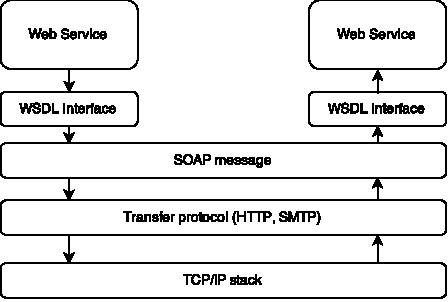
\includegraphics[width=11.5cm]{1_soap}
\caption{An example of SOAP communication}\label{soap}
\end{figure}


SOAP represents the next evolving stage between computer communication at he application layer. It was able to replace RPC technologies such as DCOM, CORBA, Java RMI. This reinstatement was highly needed because RPC technologies were brining a complex coupling to the programming language, which is definitely not a good thing. On the other hand the SOAP calls are much slower comparing to native RPC applications. There tends to be firewall latency due to the fact that the firewall is analyzing the HTTP transport. SOAP calls are much more likely to get through firewall servers, since HTTP is typically Port 80 compliant, where other calls may be blocked for security reasons. Since HTTP requests are usually allowed through firewalls, programs using SOAP to communicate can be sure that the program can communicate with programs anywhere. SOAP focuses on exposing pieces of application logic (not data) as services, platform operations. It aims for accessing named operations, each implement some business logic through different interfaces. An advantage offered by SOAP is the WS-Security which adds some enterprise security features. Supports identity through intermediaries, not just point to point (SSL). It also provides a standard for integrity.

\textbf{REST} is a simple stateless architecture that generally runs over HTTPS/TLS protocols. The flexibility is given by assigning resources their URI. The neat part is that it heavily relies on URLs. The REST philosophy is deeply entangled with HTTP protocol implementation, for instance the HTTP verbs GET, POST, PUT, DELETE, PATCH etc, are a part of REST RFC. Although it is a set of guidelines and best practices, many might understand it in their own way. Therefore, what usually happens is that the whole application is filled only with "GET" and "POST" requests. In some cases, some may even use the "GET" endpoints for creating resources, which will only confuse the reader. So this is a double-edged sword. Hence a lot of debates and discussions are still happening even today. The good part is that it doesn't need tedious descriptor files such as WSDL in order to describe a REST application. Modern frameworks usually offer a way to automatically create documentation, such as "Swagger". REST did not only impact the web architecture but it has also affected how we think about software in general. Striving to write stateless code has forever changed our mindsets, because there were times that some would think that it is absolutely fine to have methods with side effects. REST gained a lot of popularity as being a simpler alternative to SOAP and WSDL-based web services. And the most viable example is the implementation of the entire Word Wide Web. One strong thing wielded by REST applications is that the message and response content can be delivered in any format. The most used are XML based format such as HTML, and for API platforms JSON is the most common and handy format, and it has lots of advantages against XML, such as readability, payload size, easy integrable with dynamic languages, it is data oriented.

Nowadays JSON is becoming the preferred format especially for RESTful APIs. Because of the format simplicity sometimes it gets harder to define the communication structure. Which is why JSON community is working now on an elegant format called JSON-api. It simplifies a lot of things in terms of message structure. It resembles to WSDL only it is less restrictive and more intuitive. Another alternative for structuring the message format is HATEOAS. The purpose it aims is defining application state using hypertext.

\subsubsection{Data Storage}
The whole idea of computer science is wrapped around of ways of manipulating data. From the very start engineers had issues with finding ways to store data. During the time, the hardware evolved and nowadays the disk space does not represent a problem anymore. The actual challenge is how to make interaction with data as efficiently as possible. Interaction represents means of reading, and querying data, effectively saving it on the disk, keeping it consistent and avoid data loss. What if data is related to other data types. How to  implement the relationship between the data. How to make possible for multiple users to read and write at the same time. These are the actual problems which are confronted in computer science.

The classical solution to this problem are the RDBMS approaches. It is a common choice for the storage of information in new databases used for financial records, manufacturing and logistical information, personal data, and other applications since the 1980s. Relational databases have often replaced legacy hierarchical databases and network databases because they are easier to understand and use. The relational databases rely on SQL which is a special-purpose language designed for managing data. It is used to query, insert, update and modify data. RDBMS were and still are an irreplaceable solution for managing efficiently relatively small amounts of data. The RDBMS philosophy is built around ACID principle, Atomicity, Consistency, Isolation and Durability. The combination of this four principles has granted such a big success to relational databases.

As mentioned above RDBMS is widely used for lots of applications and successfully solves problems and there hasn't been a better alternative on the market. The competition is applied to different implementations of databases, such as PosgreSQL, MySQL, OracleSQL, MsSQL, MariaDB. All of them are quite similar, and each has its strong and weak points. The actual problem appears when the Big Data started to get more an more popular. Unfortunately the classical database approach was not enough for the constantly data increase. RDBMS enforces a well defined schema, as a result it gets slower and unmanageable when the amount of data gets bigger.

What developers decided was to loosen up one of the ACID principle and create new brand of databases which have a different structure and would allow storing and working with big amounts of data. This is how the term BASE principal came to life. Basically Available, Eventually Consistent. BASE concept supports the idea of network partitioning, which means that the database will always have a response disregarding the amount of requests at the given time. The catch is what kind of response should it have in case of multiple access to the database. Two solutions were proposed. First one is that the database should always return a result even though it is not up to date. The second solutions is to inform the database user that the service is not available for now. Both solutions have their own applications. Choosing which one to use depends entirely on what it is better suited for the business. The idea of choosing the database model is also presented by CAP theorem. CAP states that when choosing a database you can choose only two of the three features. These are Consistency, Availability and network Partition tolerance. In figure \mbox{\ref{cap}} is illustrated in more details the CAP and databases categorized based on theorem.

\begin{figure}[!ht]
\centering
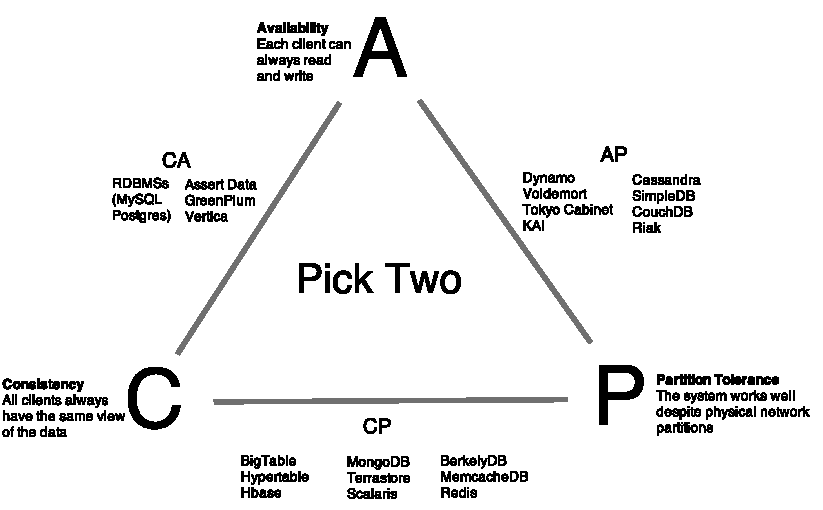
\includegraphics[width=17cm]{1_cap}
\caption{An illustration of CAP Theorem}\label{cap}
\end{figure}

Along with the implementation of conceptual new database the term NoSQL started to spread. The term came from the fact that the new databases were not using SQL for data management. In reality there are more types of conceptual database, and covering all of them under the same umbrella seems too ambiguous.
The most widely used types of databases, not considering RDBMS, are described bellow.

\textbf{Document Based Database} is a new approach of database management. It is used in usual English sense of a group of data that encodes some sort of user-readable information. This contrasts with the value in the key-value store, which is assumed to be opaque data. The basic concept that makes a database document-oriented as opposed to key-value is the idea that the documents include internal structure, or metadata, that the database engine can use to further automate the storage and provide more value.

Document databases contrast strongly with the traditional relational database (RDBMS). Relational databases are strongly typed during database creation, and store repeated data in separate tables that are defined by the programmer. In an RDBMS, every instance of data has the same format as every other, and changing that format is generally difficult. Document databases get their type information from the data itself, normally store all related information together, and allow every instance of data to be different from any other. This makes them more flexible in dealing with change and optional values, maps more easily into program objects, and often reduces database size. This makes them attractive for programming modern web applications, which are subject to continual change in place, and speed of deployment is an important issue. The current most popular implementation of such type of database is MongoDB and CouchDB.

\textbf{Column Based Database} is a database management system that stores data tables as sections of columns of data rather than as rows of data. In comparison, most relational DBMSs store data in rows. This column-oriented DBMS has advantages for data warehouses, customer relationship management systems, and library card catalogs, and other ad hoc inquiry systems where aggregates are computed over large numbers of similar data items.

It is possible to achieve some of the benefits of column-oriented and row-oriented organization with any DBMSs. Denoting one as column-oriented refers to both the ease of expression of a column-oriented structure and the focus on optimizations for column-oriented workloads. This approach is in contrast to row-oriented or row store databases and with correlation databases, which use a value-based storage structure. Such type of database implementations are BigTable, Casandra.

\textbf{Key Value Database} use the associative array (also known as a map or dictionary) as their fundamental data model. In this model, data is represented as a collection of key-value pairs, such that each possible key appears at most once in the collection. The key-value model is one of the simplest non-trivial data models, and richer data models are often implemented on top of it. The key-value model can be extended to an ordered model that maintains keys in lexicographic order. This extension is powerful, in that it can efficiently process key ranges. Example of such type of database implementations are Redis, Memcache, Voldemort.

\subsubsection{Modern Web Application}
Web applications are heavily using HTTP protocol as means of transporting data. HTTP is a stateless protocol. For every request made by a client a TCP socket is opened. The HTTP server receives a request that is handled by the application layer. When the response is sent back to the client, the TCP socket is closed and the transaction ends. The whole chain of events is repeated basically at every user interaction. The result is that a simple web application has a stateless behavior. The application layer of a web applications aims to get rid of statelessness. In 2004 the concept of web 2.0 surfaced. Javascript started to become more popular because it gave the power to animate the pages and create a more humane UX. The magic was behind the AJAX technology. The concept introduced by AJAX was making a web page run asynchronous requests and make live partially DOM changes. Developers could create web applications which did not require full page reload at while interacting with a web page. Successfully implementation of this concepts are Facebook, Gmail, Twitter etc. AJAX, JQuery and other Java Script technologies brought web applications one step closer to the desktop applications experience.

Nowadays the single page applications are becoming a hot topic. The main reason is that they are able to offer more native application like experience to the user. This is hard to do with other approaches. Supporting rich interactions with multiple components on a page means that those components have many more intermediate states. Server side rendering is hard to implement for all the intermediate states. Small view states do not map well to URLs.

Single page applications are distinguished by their ability to redraw any part of the UI without requiring a server round trip to retrieve HTML. This is achieved by separating the data from the presentation of data by having a model layer that handles data and a view layer that reads from the models. Interaction with the single page application often involves dynamic communication with the web server behind the scenes.

Here are enumerated a set of technologies that helps of building single page applications:
\begin{itemize}
    \item Ember;
    \item Angular;
    \item React;
    \item Meteor;
    \item Marionette.
\end{itemize}

Due to the fact that single page applications have a rich functionality, they also include a complex architecture. For instance in figure \mbox{\ref{ember_architecture}} is illustrated the conceptual structure of Ember framework. It is hard to wrap the head around the structure, but once there is a basic understanding of the logical layers, building applications is a joy for a developer.

\begin{figure}[!ht]
\centering
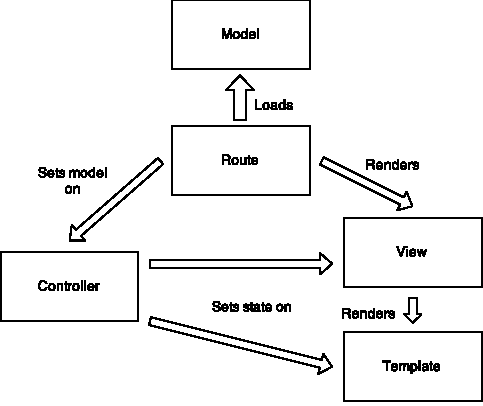
\includegraphics[width=10cm]{1_ember_architecture}
\caption{Ember framework architecture}\label{ember_architecture}
\end{figure}

But for simple applications that do not require these features, Angular or React for example might be an overkill. As new updates come out, supporting the UI might get more and more expensive. For an application with just a few buttons that the user should only interact a few times a year, simple HTML and Javascript should be just enough.

Until now everything discussed was related to building the front part of a modern web application. But a web application usually consist also from the backed part. The HTTP application that listens to client requests. For building one there are a lot of frameworks which allows to scaffold a prototype. MVC based frameworks are powerful and provides lots of functionalities out of the box and the good thing is that the majority of frameworks are mature and stable. Here are a list of frequently used solutions:
\begin{itemize}
    \item Django;
    \item ASP.NET Core;
    \item Ruby on Rails;
\end{itemize}

The mentioned technologies have huge stacks that sometimes are not needed when building a smaller application, or scalable one. Besides for building modern web applications where the client application is developed in a Javascript framework, means that the "V" (view) part from MVC is not needed anymore. Plus there are already on the market lightweight web technologies such as Sinatra, Flask, Node (in combination with express library). This type of application can serve just as good. In case if new module is required by the application, it can be easily added to the micro-framework stack. In ruby this is done by using gemfiles (gems are libraries in Ruby language) were gems can be easily added and installed effortlessly.

\subsubsection{Web Sockets}
WebSocket is a protocol providing full-duplex communication channels over a single TCP connection. The WebSocket protocol was standardized by the IETF as RFC 6455 in 2011, and the WebSocket API in Web IDL is being standardized by the W3C. The WebSocket Protocol is an independent TCP-based protocol. Its only relationship to HTTP is that its handshake is interpreted by HTTP servers as an Upgrade request. The WebSocket protocol makes more interaction between a browser and a website possible, facilitating live content and the creation of real-time games. This is made possible by providing a standardized way for the server to send content to the browser without being solicited by the client, and allowing for messages to be passed back and forth while keeping the connection open. In this way a two-way (bi-directional) ongoing conversation can take place between a browser and the server. The communications are done over TCP port number 80, which is of benefit for those environments which block non-web Internet connections using a firewall. Similar two-way browser-server communications have been achieved in non-standardized ways using stop-gap technologies such as Comet. In DSLR Camera Controller web sockets are used to transfer the live preview from the server.

The WebSocket protocol is currently supported in most major browsers including Google Chrome, Internet Explorer, Firefox, Safari and Opera. WebSocket also requires web applications on the server to support it. WebSocket reduces latency. For example, unlike polling, WebSocket makes a single request. The server does not need to wait for a request from the client. Similarly, the client can send messages to the server at any time. This single request greatly reduces latency over polling, which sends a request at intervals, regardless of whether messages are available. WebSocket makes real-time communication much more efficient. Polling can always be used (and sometimes even streaming) over HTTP to receive notifications over HTTP. However, WebSocket saves bandwidth, CPU power, and latency. WebSocket is an innovation in performance. It is also is an underlying network protocol that enables to build other standard protocols on top of it. It is also a part of an effort to provide advanced capabilities to HTML5 apps in order to compete with other platforms.
